\documentclass{article}
\usepackage{amsmath}
\usepackage{amssymb}
\usepackage{bm}
\usepackage{amsthm}
\usepackage{enumerate}
\usepackage{graphicx}
\usepackage{psfrag}
\usepackage{color}
\usepackage{url}
\usepackage{listings}
\usepackage{xcolor}
\usepackage{tikz}
\tikzset{
  treenode/.style = {shape=rectangle, rounded corners,
          draw, align=center,
        top color=white, bottom color=blue!20},
  root/.style     = {treenode, font=\Large, bottom color=red!30},
  env/.style      = {treenode, font=\ttfamily\normalsize},
  dummy/.style    = {circle,draw}
}
\definecolor{codegreen}{rgb}{0,0.5,0}
\definecolor{codewhite}{rgb}{1,1,1}
\definecolor{codegray}{rgb}{0.5,0.5,0.5}
\definecolor{codepurple}{rgb}{0.58,0,0.82}
\definecolor{codeblack}{rgb}{0,0,0}
\definecolor{codeorange}{rgb}{0.8,0.4,0}

\lstdefinestyle{mystyle}{
    backgroundcolor=\color{codewhite},   
    commentstyle=\color{codegray},
    keywordstyle=\color{codegreen},
    numberstyle=\color{codegray},
    stringstyle=\color{codeorange},
    basicstyle=\ttfamily ,
    breakatwhitespace=false,         
    breaklines=true,                 
    captionpos=b,                    
    keepspaces=true,                 
    numbers=left,                    
    numbersep=5pt,                  
    showspaces=false,                
    showstringspaces=false,
    showtabs=false,                  
    tabsize=4
}
\lstset{style=mystyle}


\setlength{\hoffset}{-0.5in}
\addtolength{\textwidth}{1.0in}
\setlength{\voffset}{-0.5in}
\addtolength{\textheight}{1.0in}
\newcommand{\be}{\begin{enumerate}}
\newcommand{\ee}{\end{enumerate}}
\newcommand{\BigO}[1]{\ensuremath\mathcal{O}\left(#1\right)}
\newcommand{\il}[1]{\lstinline!#1!}

\begin{document}
\tikzstyle{level 1}=[level distance=3.5cm, sibling distance=3.5cm]
\tikzstyle{level 2}=[level distance=3.5cm, sibling distance=2cm]
	\begin{center}
		\textbf{Spring 2020, Stats 550:\ Homework 5} \\
		\textbf{Due:\ Tuesday, February 25th, 2020} \\
		\textbf{Joseph Diaz: 819947915}
	\end{center}
\noindent\makebox[\linewidth]{\rule{\paperwidth}{0.4pt}}
\section*{Chapter 2}
\be
	\item[1.] Your friend missed probability class today. Explain to your friend, in simple
language, the meaning of \textit{conditioning}.
	\begin{proof}[Solution]
	\textit{Conditioning} is the process of determining the probability of something non-conditional in nature by considering all the probability of what could precede it and using Bayes Theorem to calculate it.
	\end{proof}
	\item[3.] Suppose $P(A) = P(B) = p_1$ and $P(A \cup B) = p_2$. Find $P(A|B)$.
	\begin{proof}[Solution]
	By the conditional probability formula:
	$$P(A|B) = \frac{P(A\cap B)}{P(B)}$$
	and by the inclusion-exclusion principle:
	\begin{align*}
	P(A\cup B) &= P(A) + P(B) - P(A \cap B)\\
	\Rightarrow  P(A\cap B) &= P(A) + P(B) - P(A \cup B)
	\end{align*}
	So the probability we are interested in is:
	$$P(A|B) = \frac{P(A\cap B)}{P(B)} = \frac{P(A) + P(B) - P(A \cup B)}{P(B)} = \frac{2p_1 - p_2}{p_1}$$
	\end{proof}
	
	\item[4.] \textbf{A paradox?} John flips three pennies.
	\be[(a)]
		\item Amy peeks and sees that the first coin lands heads. What is the probability
of getting all heads?
\begin{proof}[Solution]
Let $A$ be the event that all 3 flips are heads, and $B$ be the event that the first of the 3 flips comes heads.\\
Then the probability we are interested in is:
$$P(A|B) = \frac{P(A\cap B)}{P(B)}$$
But given that getting all heads $A$ is a subset of the event that the first coin flip is heads $B$, we may conclude: $A \cap B = A$.\\
Therefore our probability is:
$$P(A|B) = \frac{P(A)}{P(B)} = \frac{\frac{1}{8}}{\frac{1}{2}} = \frac{1}{4}$$
\end{proof}
		
		\item Zach peeks and sees that one of the coins lands heads. What is the
probability of getting all heads? (The two probabilities are different.)
\begin{proof}[Solution]
Let $A$ be the same event from part ~(a), and $C$ be the even that at least one head is flipped among the 3.
The probability of we are interested in is:
$$P(A|C) = \frac{P(A\cap C)}{P(C)}$$
To find $P(C)$, we'll use $P(C) = 1 - P(C^c)$.
If $C$ is the event where at least one head is flipped, then $C^c$ is the event where no heads are flipped at all, the probability for which is: 
$$P(C^c) = \frac{1}{8}$$
or the probability that each of the flip is tails.
So, $P(C) = 1 - \frac{1}{8} = \frac{7}{8}$.
To determine $P(A\cup C)$, we need only consider that the set of outcomes where each coin flip is heads is a subset of the event that at least one flip is heads, so:
$$A\cap C = A \implies P(A\cap C) = P(A) = \frac{1}{8}$$
Finally, our probability is:
$$P(A|C) = \frac{P(A)}{P(C)} = \frac{\frac{1}{8}}{\frac{7}{8}} = \frac{1}{7}$$
\end{proof}
			
	\ee
	\item[8.] A bag of 15 Scrabble tiles contains three each of the letters A, C, E, H, and
N. If you pick six letters one at a time, what is the chance that you spell
C-H-A-N-C-E?
	\begin{proof}[Solution]
	The probability of getting that word when sequentially picking out six letters is:
	$$\left(\frac{3}{15}\right)\left(\frac{3}{14}\right)\left(\frac{3}{13}\right)\left(\frac{3}{12}\right)\left(\frac{2}{11}\right)\left(\frac{3}{10}\right)\approx .013\%$$
	\end{proof}
	\item[10.] Box $A$ contains one white ball and two red balls. Box $B$ contains one white
ball and three red balls. A ball is picked at random from box $A$ and put into
box $B$. A ball is then picked at random from box $B$. Draw a tree diagram
for this problem and use it to find the probability that the final ball picked
is white.
\begin{proof}[Solution]
\begin{tikzpicture}
  [
    grow                    = right,
    sibling distance        = 6em,
    level distance          = 10em,
    edge from parent/.style = {draw, -latex},
    every node/.style       = {font=\footnotesize},
    sloped
  ]
  \node [root] {}
    child { node [env] {$P(R_A)$}
      child { node [env] {$P(R_B|R_A)$}
      edge from parent node [below] {Red ball $\frac{4}{5}$} }
    child { node [env] {$P(W_B|R_A)$}
      edge from parent node [above] {White ball $\frac{1}{5}$} }
      edge from parent node [below] {Red ball $\frac{2}{3}$} }
    child { node [env] {$P(W_A)$}
      child { node [env] {$P(R_B|W_A)$}
      edge from parent node [below] {Red ball $\frac{3}{5}$} }
    child { node [env] {$P(W_B|W_A)$}
      edge from parent node [above] {White ball $\frac{2}{5}$} }
      edge from parent node [above] {White ball $\frac{1}{3}$} };
\end{tikzpicture}\\
Using the above tree diagram, we have that:
\begin{align*}
P(W_B) &= P(W_B|W_A)P(W_A) + P(W_B|R_A)P(R_A) \\
&= \frac{2}{5}\cdot\frac{1}{3} + \frac{1}{5}\cdot\frac{2}{3}\\
&= \frac{4}{15}
\end{align*}

\end{proof}	
	\item[12.] Suppose $P(A) = 1/2, P(B^c|AC) = 1/3$ and $P(C|A) = 1/4$. Find $P(ABC)$.
	\begin{proof}[Solution]
	Using Bayes Theorem, we have:
	$$P(A\cap C) = P(C|A)P(A) = \frac{1}{2 \cdot 4}=\frac{1}{8}$$
	And by the law of total probabilities and, again, using Bayes Theorem:
	\begin{align*}
	P(A\cap C) &= P(A\cap C|B^c)P(B^c) + P(A\cap C|B)P(B)\\
	&= \frac{P(A\cap C\cap B^c)P(B^c)}{P(B^c)} + \frac{P(A\cap C\cap B)P(B)}{P(B)} \\
	&= P(A\cap C\cap B^c) + P(A\cap C\cap B)\\
	\Rightarrow P(A\cap B\cap C) &= P(A\cap C) - P(A\cap C\cap B^c)\\
	&= P(A\cap C) - P(B^c|A\cap C)P(A\cap C)\\
	&= \frac{1}{8} - \frac{1}{3}\cdot\frac{1}{8}\\
	&= \frac{1}{12}
	\end{align*}
	So:
	$$P(A\cap B\cap C) = \frac{1}{12}$$
	\end{proof}
	
	\item[17.] Amy has two bags of candy. The first bag contains two packs of M\&\!\! Ms and
three packs of Gummi Bears. The second bag contains four packs of M\&\!\! Ms and two packs of Gummi Bears. Amy chooses a bag uniformly at random and
then picks a pack of candy. What is the probability that the pack chosen is
Gummi Bears? Solve (i) by using a tree diagram and (ii) by another method.
	\be[(i)]
		\item 
		\begin{proof}[Solution]
		With Law of Total Probabilities:\\
		Let $G$ be the event that you get a pack of Gummi Bears and $M$ be the event that you get a pack of M\&\!\! Ms, and $A$ and $B$ be the event that you pick the first or second bag, respectively. Then the probability of getting Gummi Bears is:
		\begin{align*}
		P(G) &= P(G|A)P(A) + P(G|B)P(B)\\
		&= \frac{3}{5}\cdot\frac{1}{2} + \frac{1}{3}\cdot\frac{1}{2}\\
		&= \frac{7}{20}
		\end{align*}
		\end{proof}
		
		\item 
		\begin{proof}[Solution]
		With a tree diagram:\\
		\begin{tikzpicture}
  [
    grow                    = right,
    sibling distance        = 6em,
    level distance          = 10em,
    edge from parent/.style = {draw, -latex},
    every node/.style       = {font=\footnotesize},
    sloped
  ]
  \node [root] {}
    child { node [env] {$P(B)$}
      child { node [env] {$P(G|B)$}
      edge from parent node [below] {Gummi Bears $\frac{1}{3}$} }
    child { node [env] {$P(M|B)$}
      edge from parent node [above] {M\&\!\! Ms $\frac{2}{3}$} }
      edge from parent node [below] {Bag $B$ $\frac{1}{2}$} }
    child { node [env] {$P(A)$}
      child { node [env] {$P(G|A)$}
      edge from parent node [below] {Gummi Bears $\frac{3}{5}$} }
    child { node [env] {$P(M|A)$}
      edge from parent node [above] {M\&\!\! Ms $\frac{2}{5}$} }
      edge from parent node [above] {Bag $A$ $\frac{1}{2}$} };
\end{tikzpicture}\\
And from this diagram we have:
$$P(G) = \frac{3}{5}\cdot\frac{1}{2} + \frac{1}{3}\cdot\frac{1}{2} = \frac{7}{20}$$
		\end{proof}
	\ee
	
	\item[22.] Consider flipping coins until either two heads $HH$ or heads then tails $HT$ first
occurs. By conditioning on the first coin toss, find the probability that $HT$
occurs before $HH$.
\begin{proof}[Solution]
The probability that one event happens before another is given by:
$$\frac{P(HH)}{P(HT) + P(HH)}$$
which equals:
$$\frac{\frac{1}{4}}{\frac{1}{4}+\frac{1}{4}} = \frac{1}{2}$$
\end{proof}
	
	\item[23.] In a certain population of youth, the probability of being a smoker is 20\%.
The probability that at least one parent is a smoker is 30\%. And if at least
one parent is a smoker, the probability of being a smoker is 35\%. Find the
probability of being a smoker if neither parent is a smoker.
	\begin{proof}[Solution]
	Let $P(S) = 1/5$ be the probability that a youth is a smoker, $P(M) = 3/10$ be the probability that one or more parents of a youth smokes, and $P(S|M) = 7/20$ be the probability that a youth is a smoker given that at least one parent is a smoker. Then the total probability that a youth is a smoker is:
	$$P(S) = P(S|M)P(M) + P(S|M^c)P(M^c)$$	
	Then the probability that a youth smokes given that neither parent smokes $P(S|M^c)$ is given by:
	\begin{align*}
	&P(S) = P(S|M)P(M) + P(S|M^c)P(M^c)\\
	&P(S|M^c)P(M^c) = P(S) - P(S|M)P(M)\\
	&P(S|M^c) = \frac{P(S) - P(S|M)P(M)}{P(M^c)}\\
	&\qquad = \frac{\frac{1}{5}- \frac{7}{20}\cdot\frac{3}{10}}{\frac{7}{10}} = \frac{19}{140} \approx 13.57\%
	\end{align*}
	\end{proof}
	\item[25.] A polygraph (lie detector) is said to be 90\% reliable in the following sense:
There is a 90\% chance that a person who is telling the truth will pass the
polygraph test; and there is a 90\% chance that a person telling a lie will fail
the polygraph test.
	\be[(a)]
		\item Suppose a population consists of 5\% liars. A random person takes a polygraph
test, which concludes that they are lying. What is the probability
that they are actually lying?
		\begin{proof}[Solution]
		Let $T$ and $T^c$ be the events that a person is a truth teller or liar, respectively, and $C$ and $C^c$ be the event that a person passes or fails the polygraph. Then $P(C|T) = .9,\ P(C^c|T^c) =.9\ P(C^c|T) = .1,\ P(C|T^c) =.1$ and $P(T) = .95,\ P(T^c) =.05$.\\
		Then the probability that a person is lying given that they failed the polygraph is:
		\begin{align*}
		P(T^c|C^c) &= \frac{P(C^c|T^c)P(T^c)}{P(C^c)}\\
		&= \frac{P(C^c|T^c)P(T^c)}{P(C^c|T^c)P(T^c)+P(C^c|T)P(T)}\\
		&= \frac{.9\cdot .05}{.9\cdot .05+.1\cdot.95}\\
		&= .321
		\end{align*}
		So the probability is about 32\%.
		\end{proof}
		\item Consider the probability that a person is actually lying given that the polygraph
says that they are. Using the definition of reliability, how reliable
must the polygraph test be in order that this probability is at least 80\%?
\begin{proof}[Solution]
If we take the expression from part ~(a):
$$\frac{P(C^c|T^c)P(T^c)}{P(C^c|T^c)P(T^c)+P(C^c|T)P(T)}$$
and let $P(C^c|T^c) = x$ and also recognize that $P(C^c|T) = 1 - P(C^c|T^c)$; then we can set the expression equal to the probability that we want and determine the \textit{reliability} that would yield that probability:
\begin{align*}
&\frac{xP(T^c)}{xP(T^c)+(1-x)P(T)} = \frac{8}{10}\\
&10xP(T^c) = 8xP(T^c) + 8P(T) - 8xP(T) \\
&x(2P(T^c) + 8P(T)) = 8P(T)\\
&x = \frac{8P(T)}{2P(T^c) + 8P(T)} \approx 98.7\%
\end{align*}
So the test would need to be 98.7\% reliable.
\end{proof}
		
	\ee
	\item[28.] The R command \il{sample(1:365,23,replace=T)} simulates birthdays from a group of 23 people. The expression \il{2 \%in\% table(sample(1:365,23,replace=T))} can be used to simulate the birthday problem. It creates a frequency table
showing how many people have each birthday, and then determines if two is
in that table; that is, whether two or more people have the same birthday. Use
and suitably modify the expression for the following problems.
	\be[(a)]
		\item Simulate the probability that two people have the same birthday in a room
of 23 people.
\begin{lstlisting}[language=R]
n = 1000
sim = replicate(n, if(2 %in% table(sample(1:365,
 				23, replace=T))) 1 else 0)
mean(sim)
# 0.487
\end{lstlisting}
The probability is about 49\%.
		\item Estimate the number of people needed so that the probability of a match
is 95\%.\\\\
\textit{Solution.}\\
Intuitively, we would expect the likelihood of a matched birthday to double if we double the number of people that we query. So retrying the simulation with about double the number of people produces what we're interested in:
\begin{lstlisting}[language=R]
n = 1000
sim = replicate(n, if(2 %in% table(sample(1:365, 
				48, replace=T))) 1 else 0)
mean(sim)
# 0.954
\end{lstlisting} 
So sampling around 50 people gives a probability of about 95\% that two people share a birthday.\\
		\item Find the approximate probability that three people have the same birthday
in a room of 50 people.
\begin{lstlisting}[language=R]
n = 1000
sim = replicate(n, if(3 %in% table(sample(1:365, 
				50, replace=T))) 1 else 0)
mean(sim)
# 0.114
\end{lstlisting}
The Probability if about 11\%.
		\item Estimate the number of people needed so that the probability that three
people have the same birthday is 50\%.\\\\
\textit{Solution.}\\
Unlike part ~(b), we only needed to just about double the number of people sampled to quadruple the probability:
\begin{lstlisting}[language=R]
n = 1000
sim = replicate(n, if(3 %in% table(sample(1:365, 
				90, replace=T))) 1 else 0)
mean(sim)
# 0.502
\end{lstlisting}
So around 90 people must be sampled for the probability of 3 matched birthdays to be around 50\%.
	\ee
	
	\item[29.] Simulate the nontransitive dice probabilities in Exercise 2.6.\\\\
\textit{Solution.}\\
The following R code simulates the experiment:
\begin{lstlisting}[language=R]
n = 1000
# Number of trials
dA = c(3,3,5,5,7,7)
dB = c(2,2,4,4,9,9)
dC = c(1,1,6,6,8,8)
# The above vectors simulate the non-standard dice

mean(sample(dA, n, replace = T) > 
		sample(dB, n, replace = T))
# 0.57

mean(sample(dB, n, replace = T) > 
		sample(dC, n, replace = T))
# 0.571

mean(sample(dC, n, replace = T) > 
		sample(dA, n, replace = T))
# 0.569
\end{lstlisting}
The commented probabilities are consistent with the expected probabilities from the original question.

\ee
\noindent\makebox[\linewidth]{\rule{\paperwidth}{0.4pt}}
	
\end{document}
